\documentclass[a4paper]{report}
\title{Using fNIRS to Detect Mental Workload and Emotional Valence in web form filling task}%changing the layout of long web forms
\date{2015-09-18}
\author{Kristiyan Lukanov}
\usepackage{graphicx}
\usepackage{amsmath}
\usepackage{url}
\usepackage{color,soul}
\usepackage{caption} 
\captionsetup[table]{skip=10pt}
\renewcommand{\bibname}{References}
\renewcommand{\arraystretch}{1.3}
\begin{document}
\pagenumbering{gobble}
\maketitle
\newpage
\pagenumbering{arabic}

\section*{Acknowledgements}
lorem ipsum 
\newpage
	
\section*{Abstract}
In this dissertation we evaluated a desktop interface using functional near infrared spectroscopy(fNIRS), and verified the practicality of this brain imaging modality. More specifically, we tested the web page layout of online insurance claim process...
\newpage
\tableofcontents
\newpage
	
\chapter{Introduction}
	%The whole thesis should be third person past tense. Participants were asked to read and sign

	Users often has to fill web pages containing more than 10 forms for example, when registering for a web site, posting classified ad, or sending online insurance claim. Sometimes this is really important in Human computer interaction(HCI) viewpoint, like filling insurance claim forms, and online banking to be intuitive and aiding the user through the process. To achieve that web forms should support the users working memory\cite{nielsen1990heuristic,shneiderman1992designing} by minimizing the effort to perceive, process and respond to the web form. That is why we are interested in measuring the mental demands imposed by the web form filling task. Furthermore, it has been suggested that attractive interfaces increase creativity\cite{norman2002emotion} of the user. Hence, it can be of high value for the researchers to know what workload and emotional state the users are experiencing during interaction with a certain interface.
	
	Recently, functional near infrared spectroscopy(fNIRS) has been suggested as a suitable brain imaging method for HCI studies\cite{maior2015examining,solovey2009using,pike2014measuring} because participants can wear it during normal interaction with a computer interface. In addition, the brain scanning device is non-intrusive and relatively resistant to motion artefacts which will not affect task performance and data collected, in contrast to other brain imaging modalities. Moreover, as it has been suggested by cognitive neuroscience studies that the prefrontal cortex(PFC) area of the brain is involved with higher order cognition\cite{braver1997parametric} and emotion processing\cite{damasio1996somatic}. Thus, by placing the fNIRS device on the forehead of individuals we can infer about their level of demand and emotional state.
	
	However, according to our knowledge only one study was found\cite{peck2013using} that uses hemodynamic data from fNIRS to compare and evaluate different variations of an interface. Other fNIRS studies experiment with simple tasks, like mental arithmetic, and n-back tasks. Accordingly, we want to implement the fNIRS device in a user trial evaluation study of an web interface because it is often encountered task in our daily lives. 
	
	\section{Purpose of study}
		 We aim to find a way to improve web interfaces that has more than 10 forms, and are considered long forms, as this process is often encountered during daily web surfing, for example, when user registers to a new web site, or enter information for financial institutions, like insurance companies and banks. We strive to find more generalizable results that can produce certain web form design guidelines for interacting with long forms. Accordingly, we decided to test the layout of the web forms, and examine how it influences user performance. We also, aim to assess the practicality of fNIRS brain imaging technique in HCI evaluation studies.
	\section{Research questions}
		In this master thesis we aim to answer the following questions:
		\begin{enumerate}
			\itemsep0em
			\item Which of the three layouts elicit the least mental workload and which is more preferred by the users?
			\item Is fNIRS sensitive method in measuring mental workload changes in web form filling task? 
			\item Can we detect emotional valence with fNIRS, from web interface that has no emotional cues.
			\item Is fNIRS brain imaging modality practical to use in HCI evaluation studies?
		\end{enumerate}		
	\section{Industry partner}
		This work has been motivated by the need of entity partner funding my masters course. The industry partner operates an insurance customer relationship management(CRM) software, and it was requested to provide insights in the web form filling process and provide design guidelines.	
	\section{Structure of the thesis}
		In the next chapter we will first review the background literature behind usability and web form filling, the concept of mental workload and working memory, emotion processing, and finally, relevant brain sensing techniques. In chapter 3 we will describe the User study, including description of the method we used, and the results obtained. Finally, we will discuss the finding from the experiment and then propose implications for design.
\chapter{Literature review}
	In the HCI field  evaluation approaches ca be divided in three general categories: analytical, field study and lab study\cite{rogers2007interaction}. First, analytical methods are designed to predict user behaviour such as, heuristic evaluation or expert reviews, so no experiment has to be conducted. Second, field studies are conducted in context in order to collect relevant and valid data, like observations. Lastly, lab studies use artificial settings but the experiment variables can be controlled easier, and also, comparative tests can be conducted. Our aim of the study is to evaluate a web form filling interface for the insurance domain, and more precisely, online auto insurance claim process. Therefore we are interested in conducting lab study because we cannot simulate road accident and we are able to compare variations of insurance claim web form. Furthermore, there are variety of evaluation methods, like interviews which will give us information about what users think about the interface, or observations which will let us recognize typical behaviour of users and obstacles they encounter while using the interface.\\
	
	It has to be mentioned that lab studies give us the chance to prepare the environment and record more performance measures which provide valuable objective information. Typical performance measures in usability experiments are time to complete, errors encountered, and number of events. In general, mental workload and emotional valence are of high interest in HCI evaluations because measuring workload gives us important information about the task demands and also, knowing whether a user is feeling positive or negative towards an interface or task may give us valuable information about their general preferences. Furthermore, Nielsen\cite{nielsen1994measuring} suggested that user preferences correlate with user performance, thus we can rely solely on user preferences, however this is not always the case. Hence, Nielsen and Levy \cite{nielsen1994measuring} advise researchers to use combination of subjective and objective data in usability studies, in order to identify bias and provide richer information about the process. Accordingly, we have decided to employ user trials(subjective data) combined with psychophysiological measurements(objective data). In addition, functional near infrared spectroscopy (fNIRS), has been recently suggested as a promising method for HCI evaluations\cite{maior2015examining,pike2014measuring} because it was suggested to measure mental workload\cite{maior2014continuous}. Based on this, we decided to test the usefulness of fNIRS in HCI evaluation studies. \\
	
	Based on the information above this master thesis considers measuring mental workload and emotional valence to inform the user interface design of the insurance claim web form. The literature review will proceed in the following way: first, we will review relevant literature on web form filling and usability. Second, we discuss working memory models and the mental workload concept. Third, emotional processing literature will be revised. Fourth, current brain sensing techniques used in cognitive experiments will be reviewed and, fifht, fNIRS studies examining mental workload and emotional valence will be examined. Finally, we will summarize the reviewed literature. 
	
	\section{Usability and Web form filling}	
		Web form filling is often encountered activity in daily surfing of web users, however, according to our knowledge, there is scarce of empirical research in the Human Computer Interaction(HCI) literature for this topic. First, a study by Wästlund\cite{Wastlund20081229} compared two web page layouts - one that all the text is in the same page, and one where the text is separated in four pages. Authors concluded that users experienced less workload with the divided web form(4 pages), compared to the single page web form. Second, two books specially written for web form filling design\cite{jarrett2009forms,wroblewski2008web} suggest splitting long web forms into several pages, in order to improve the process. Lastly, most of the research on web form filling and design is focused in optimizing the experience and accessibility for elderly population\cite{sayago2012selective,chadwick2003web,lines2006online,sayago2007some}.
		
		In reviewing positive and negative affect and their implications for design Norman\cite{norman2002emotion} proposes that ``Positively valenced affect broadens the thought processes hence, enhanced creativity''. Therefore, increase in task performance should be observed when a user has positively valenced affect towards certain interface. Suggesting that emotional valence plays pivotal role in task performance. Also, A couple of studies suggest that the longer it takes for a task(short or long term) to be completed the more the perceived frustration the users experience increases\cite{mendoza2005usability,bessiere2004social}. Therefore, we should aim to minimize frustration by reducing the time to complete a task.
			
		Because of insufficiency of relevant literature on the web form filling and design we are going to examine general usability guidelines and recommendations as they are widely accepted by the Human Computer Interaction researchers. The two most popular usability heuristics are those of Nielsen\cite{nielsen1990heuristic}, and Shneidermann\cite{shneiderman1992designing}. They express similar suggestions, like, maintain consistency, provide feedback, support expert users, prevent and optimize error messages, provide help documentation, permit easy reversal of information, and minimize working memory load. Consequently, the design of the tested variants in the usability study in chapter 3 is informed by them. Also, because both heuristics advocate minimizing the load on working memory we consider that reducing it will provide better user experience. In addition, because usability of certain interface depends on the context, user differences, and that there is not perfect solution to a interface problem, and designers often have to make tradeoffs\cite{norman1986user}, we will rely on cognitive science in order, to predict which layout is more appropriate.

	\section{Working Memory and Mental Workload}
		The concept of mental workload (MW) is intuitive in nature and it represents how busy an operator is when performing a certain task. The concept has been referred in the literature with many terms, like cognitive load, stress, strain, and arousal. Many definitions has been proposed by many authors, however researchers are still unable to find a consensus on the term[Linton et al 1989]. Wickens\cite{wickens2008multiple} defines it as ``The demand imposed by tasks on the human's limited resources, whether considered single or multiple''. Depending on the studied task at hand, knowing workload experienced by different design variations will help choose the one that generates desired operator performance. Also, in terms of operator experience of MW, Rouse et al classifies different factors like, fatigue, mood, individual differences, as person-specific workload\cite{rouse1993modeling}. Similarly, Norman and Bobrow classified operator performance on data-limited and resource-limited\cite{norman1975data}. They hypothesize that even if operator spends high amount of attentional resources, the task can have a bad representation that will degrade the performance. In contrast, resource-limited performance depends on how much attentional resources the task demands, and it can be considered that every real life task consists of combination of both. 
			\subsection{Working memory models}
			Rather than searching for definition researchers in cognitive science use models of working memory in order to understand cognition, predict and explain workload and performance. Furthermore, theories of working memory try to define the processes going into human mind, and explain concepts such as, attention, perception, long term memory, decision making, action selection, and execution\cite{wickens-1988,baddeley1974working,miller1956magical}. 			Most of those models are based on human as information processor approach \cite{broadbent1,broadbent2,neisser,wickens-1988}, which relates the processes of human mind with those of a computer processor. Also, the framework is based on the assumption that the human operator has a limited resource capacity\cite{kahneman1973attention,wickenshollands1999} and if the task demands more resources than the capacity of the operator, workload overload is observed. Moreover, the information from the environment or the task is processed by series of processing systems, like perception, attention, short-term memory, long-term memory.			
			\begin{figure}[h]
				\centering
				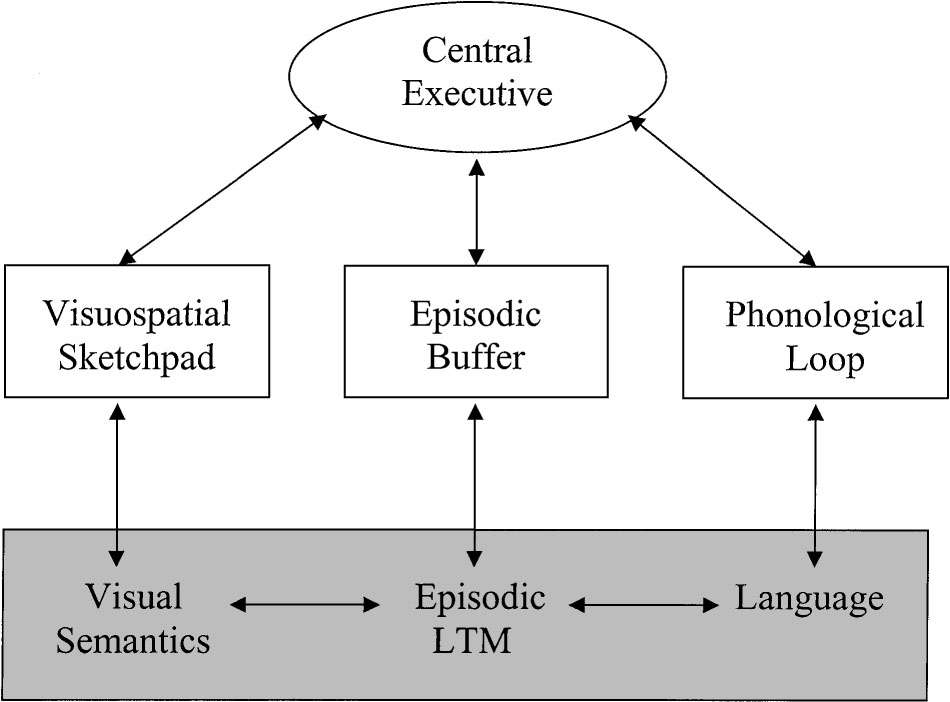
\includegraphics[width=0.7\linewidth]{baddeley-wm}
				\caption[Baddeley and Hitch Working memory model]{Working memory model by Baddeley and Hitch, displaying the 'slave systems' visuo-spatial sketch pad, episodic buffer and phonological loop, controlled by the central executive.}
				\label{fig:baddeley-wm}
			\end{figure} 
		
			In attempt to describe the web form filling task we can use the working memory model from Baddeley and Hitch \cite{baddeley1974working} which processes information in verbal and spatial form . It consists of a central executive, which is acts as an administration system which controls the information input and output of its slave systems. The visuo-spatial sketch pad is involved in holding visual information in spatial form like, objects and colours. The phonological loop stores verbal information, such as words and names. 			And the later proposed \cite{baddeley2000episodic} episodic buffer is responsible for the storage and retrieval of memories or events. Because the task of web form filling involves multiple cognitive processes like, visual search, speech synthesis, planning, memory retrieval, decision making, thus utilizing all slave systems of the model, we can label the web form filling process as one that involves complex cognition. 		
			\begin{figure}[h]
				\centering
				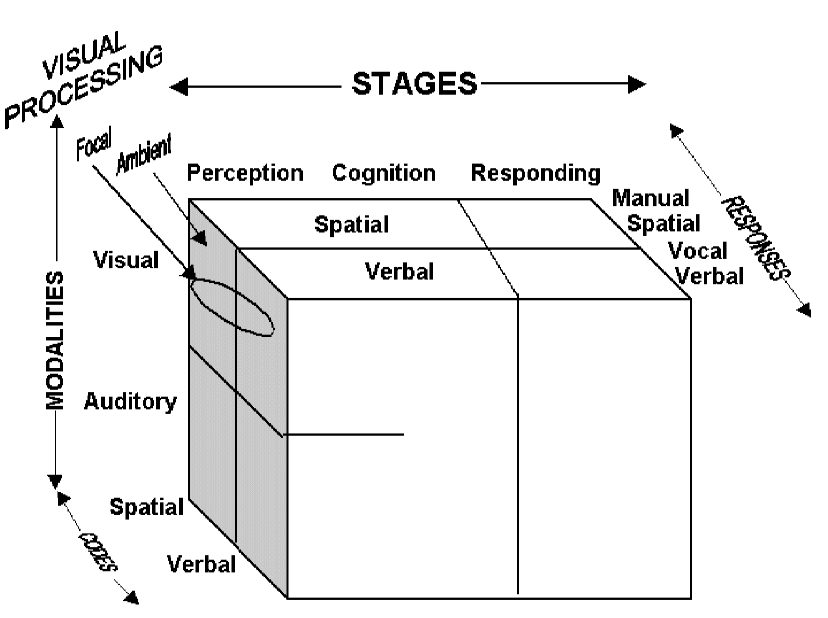
\includegraphics[width=0.8\linewidth]{mrt}
				\caption[Multiple resource theory by Wickens]{Wickens 4-D multiple resources model consisting of two codes(spatial and verbal), 2 modalities(auditory and visual), 3 stages(perception, cognition and responding), and 2 types of responses(manual and vocal).}
				\label{fig:mrt}
			\end{figure}
			We can also consider the multiple resources model by Wickens\cite{wickens2008multiple,wickens2002multiple} which is suited for predicting the workload of an operator performing multiple tasks at one time. The 4-D multiple resources model is visualised as 4 dimensional cube as illustrated in Figure \ref{fig:mrt}.The approach is based on four basic assumptions:

			\noindent1) in the stages of processing dimension, perceptual and cognitive tasks use different resources than response selection and execution;\\
			2) spatial activity uses different resources than verbal or linguistic activity;\\
			3) the modalities dimension, different resources are used for auditory and visual perception\\
			4) visual channels are divided on focal and ambient vision\\
			And the main argument of the theory is ``to the extent that two tasks use different levels along each of the three dimensions, time-sharing will be better'' \cite{wickens2008multiple}. The model provides an account on how different elements of the human information processor, like attention, perception, working memory, response selection and execution interact between each other. This theory is also based on research from cognitive neuroscience that suggests  different modalities have different locations in the human brain, like the auditory cortex is involved with auditory perception and the visual perception is processed mainly by the visual cortex(occupational lobe).\\

			However, mental workload can be influenced by the initial perception of the task at hand or the 'appraisal' of it. Similarly to MW appraisal is complex and multidimensional concept\cite{folkman1986dynamics,peacock1990stress} that is not well defined.
		
			\subsection{Measuring Mental Workload}
			The concept has been explained differently by different authors, and inferences made from various empirical measures which can be divided on primary, secondary, subjective and psychophysiological measures. There are also analytical techniques but we are not concerned with them in this dissertation.
				\subsubsection{Primary and secondary task measures}
				Primary measures rely on operator performance to predict workload. However, a limitation of using primary measures alone is that an operator can spend high amount of effort but this may not be apparent from the performance\cite{wilson2015evaluation}. Consequently, primary task measures should be combined with other workload measures. An example performance measures are task completion time, number of errors, and response time. In our case we will use a combination of all but secondary task measures. Secondary task involves inclusion of a additional simple task to the primary one, which is done concurrently, if the primary task has low or moderate demand and the level of workload cannot be inferred only from the primary measure. It is used to detect when operators performance deteriorates and this is due to workload overload. However, as we are not going to use secondary measures, more explanation will provided for the other types of measurements.
				\subsubsection{Subjective measures}
				Subjective measures use rating scale and are based on operator opinion of their perceived workload during or after completion of task. They are preferred method for WL estimation because they are easy to administer, cheap, and with high face validity. They are classified as uni dimensional and multidimensional. They consist of single subjective scale of workload and multiple scales of types of workload, accordingly. From the unidimensional subjective measures the Cooper-Harper\cite{cooper1969use} is the most popular among ergonomists and cognitive researchers. However, it is designed for the aircraft domain, and therefore a modified cooper-Harper scale\cite{wierwille1983validated} was created for use in other domains. However, as mental workload is influenced by different environmental and personal factors\cite{rouse1993modeling}, therefore the concept of MW should be considered as multidimensional concept, in order to improve diagnosticity. Accordingly, multi-dimensional subjective scales should be used to better understand the aspects of MW. The most used scales are NASA-TLX\cite{nasatlx}, SWAT\cite{reid1988subjective} and Workload profile\cite{tsang1996diagnosticity}. NASA-TLX is based on rigorous laboratory research, and it includes 6 scales (mental, physical, temporal demand, experienced effort, frustration and performance) consisting of 20 intervals each and it is relatively easy to administer. In addition, a single measure of workload can be weighted, although it is not necessarily required because there is high correlation between weighted and unweighed results\cite{byers1988workload}. 
				The SWAT subjective scale is also widely used, however the process of implementation is laborious and more complex than the other subjective scales. The other popular scale is Workload profile(WP)\cite{tsang1996diagnosticity} scale which is basen on the Wickens multiple resources model, and asks questions about each of the four dimensions proposed by the theory. Hence, it is very useful when combined with multiple resource theory interpretation of the results. Finally, Longo et al. \cite{longo2012importance} compared the three measures mentioned above in a web browsing/searching task, and observed correlations in the results of the three measures claiming that they measure the same concept of mental workload.\\
				\subsubsection{Psychophysical measures}
				Psychophysical measures are used to give objective data about mental workload by not relying on subjective scales or performance measures . They can be obtained by recording cardiac activity, electrodermal activity, eye function or imaging the brain. These techniques detect the  change in the arousal from the autonomic nervous system level which can be inferred to as mental workload. However, different psychophysical measures capture different aspects mental workload\cite{cain2007review}, therefore consideration should be put in choosing the most appropriate measure for the given task. \\
				Mean heart rate(HR) and heart rate variability(HRV) are one of the most used techniques to infer arousal because it is relatively cheap and easy to administer. However, HR not always correlates to subjective measures of MW\cite{haapalainen2010psycho} and because of this HRV can be considered as more valid measure. Moreover, the beat to beat interval of the heart can be measured using different statistical approaches\cite{billman2011heart}, like, standard deviation from heart beat intervals. Measurements of eye activity, like blink rate, pupil diameter are also being found to correlate to MW. Furthermore, increase in pupil diameter is correlated to rise in arousal \cite{kahneman1973attention}, and Beatty claimed that it has high sensitivity \cite{beatty1982task} and it can be used to distinguish between data-limited and resource limited processing, which can make it very useful in the HCI field. However, incoming light at the eye can change the pupil diameter, which is a process unrelated to the task, thus influencing the measurements, therefore it is suitable for experiments in controlled environment. \\Finally, a number of brain imaging techniques are used to obtain measurements from the brain activity, including electroencephalography(EEG), functional near-infrared spectroscopy(fNIRS), functional magnetic resonance imaging(fMRI), however these will be discussed later in section "Brain sensing".
		
		 %and yielded similar results, suggesting they measure the same aspects of the web task. The author infers that only one mental workload measure is required. Because mental workload is influenced by a number of factors, and therefore it is multidimensional concept, NASA-TLX is chosen as subjective measure for the experiment.
		
 
		 %Lavie(2005,2010) Load theory says high perceptual load decreases attention to distractions, and low perceptual load increased them. High perceptual load is experienced when, for example, driving fast a car, or playing sports. Furthermore, because it involves a lot of perceptual capacity there is no spare capacity for the attention to perceive distractions. In this case, the task has a low perceptual load because it demands only to a visual stimuli to be percieved and processed rather than with audioty, o

	\section{Emotion processing}
		To begin with, mood and emotion are frequently referred as separate concepts. For example, emotions are thought to last for shorter time like, several minutes, in comparison to moods which can last for a whole day or more. Also, emotions are generally caused by certain events, like winning a game, in contrast to moods where often there is no reason as to why an individual is in certain mood. However, there is no clear distinction between them because moods can cause certain emotions and emotions can cause moods. To solve that problem researchers often use the term ``affect'' to encompass both emotions and moods. Furthermore, we can define positive moods or emotions as positive affect, and negative emotion and moods as negative affect.
		
		There are two major approaches in describing emotions - the categorical\cite{izard2007basic} and the dimensional approach\cite{feldman1998independence}. The first one, categorises several different emotions like, happiness, sadness, anger, fear, and disgust, and often matches the subjective experience of individuals. The second one, the dimensional approach considers emotions to have two distinct dimensions of pleasure-misery (emotional valence) and arousal-sleep.  
		\begin{figure}
			\centering
			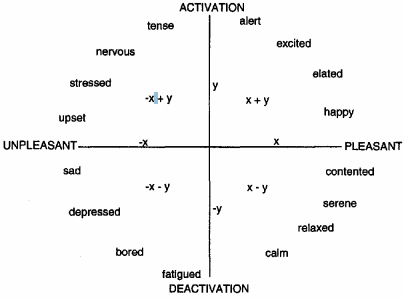
\includegraphics[width=0.7\linewidth]{two-demensional-approach-emotions}
			\caption[Two dimensional approach of emotion]{The two dimensional approach of emotion. The x and y axes represent semantic components: x=pleasant and unpleasant emotions, and y=level of activation. The image is taken from Russell and Feldman ``Independence and bipolarity in the structure of current affect''\cite{feldman1998independence} }
			\label{fig:two-demensional-approach-emotions}
		\end{figure}
		For example, the happy emotion can be pointed to have high positive valence and moderate activation or arousal. In contrast, the emotion of sadness has high negative valence and again moderate arousal. Furthermore, there is a considerable debate on which approach should be adopted by researchers\cite{fox2008emotion}, however we decided to use the dimensional approach because we wanted to have a numerical measure of emotional valence, which than can be compared to the objective data.
		
		Also, emotion processing depends on top-down(appraising a situation based on similar previous knowledge) and bottom-up(processing external stimuli) processes. The first one(top-down) is more cognitive process because it uses attention and memory in order to assign a valence to a given stimuli. The bottom up processing is influenced by external stimuli, so it uses more visual perception. Generally, there are considerable differences between them, and many theorists considers which one of them is more involved with emotion generation. However, there are many ``appraisal theories'' that suggest cognition strongly influences when we experience emotional states and what particular states we experience in a certain moment. For instance, one can appraise a non-threatening situation as threatening and therefore she will experience negative valence. Moreover, many theorists argue that appraisal is both conscious and automatic. Smith and Kirby\cite{smith2009putting} suggested two types of appraisal: one that is based on reasoning(deliberate thinking), and one that is based on activation of memories(automatic processes). The first one is claimed to be slower and more flexible. 
		
		It has been assumed that emotional states influence cognition\cite{blanchette2010influence}, like attention, perception, decision making, and others. Also, what we remember from a situation is strongly affected by what we attended during that time\cite{eriksen1986visual}. In addition, an influential theory by Easterbrook\cite{easterbrook1959effect} suggest the number of attentional cues processed declines as arousal or anxiety increases. It can be interpreted as strong negative valence causes "tunnel vision", and positive valence produces breadth of attention. For example, a individual in highly stressful situation, like auto mobile incident, will remember only the low amount of details related to the moment of the accident. In contrast, when one is experiencing positive situation, it is likely that she will remember more unrelated details about the event. However, Harmon-Jones et al.\cite{harmon2011toward} argued that the above mentioned theory considering only emotional valence is over simplified and it lacks the addition of \textit{motivational intensity}. Generally, there are two types of motivation: approach and avoidance motivation. According to the authors the approach motivation can be low, for example listening to music, or high, for instance recognizing a attractive subject from the opposite sex. On the other hand, low avoidance motivation can be exposure to unfair situation, and high avoidance motivation can be dealing with life-threatening situation. Harmon-Jones et al.\cite{harmon2011toward} postulated that high motivational intensity leads to narrowing of the attention for both positive and negative experiences because it helps individuals to successfully accomplish tasks. On the contrary, low motivational intensity for both positive and negative experiences leads to attentional broadening because individuals leave spare attentional resources, in order to be able to encounter and react accordingly to a new and maybe more valuable situation.
		
		Russell\cite{russell2003core} proposed a valence model of emotion which states that significant higher activation of the left hemisphere compared to the right was associated with positive emotions, whereas significantly higher activation in the right hemisphere should be associated with negative emotion. Therefore, we can infer whether an affect was positive or negative if we measure the brain activation during an experiment.
		
		Generally, there are two methods that are widely used for measuring affect: objective and subjective. One subjective measurement technique is the self assessment manikin(SAM)\cite{bradley1994measuring}, which we used because it provides two scales - emotional valence and arousal. Other widely used measure is the Positive and Negative Affect Schedule(Panas)\cite{watson1988development}. However, it is more complex to use, for example, explain to participants how to use it, and also, the procedure takes more time. However, we want to avoid that because of the increasing uncomfortability of wearing fNIRS device with the time. Also, the scales had visual icons that help participants recognise what each point of the scale means. The objective techniques that try to infer emotional valence include psychophysiological measures of galvanic skin response, heart rate, respiration\cite{krumhansl1997exploratory}, and brain activity\cite{Balconi201567}. We decided to combine subjective and objective measure of emotional valence, in order to compare them and later make inferences about. We chose SAM because it is widely accepted, and easy to implement, and brain sensing technique for the objective measure, as we try to prove the left vs right hemisphere hypothesis of Davidson\cite{davidson1992emotion} which is explained below. Next, we will review brain sensing techniques and pick one suitable for this master thesis experiment.
		
		%10. mood congruity
		%11. Dual process model - fast automatic and affective system and slower effortful and more cognitive system
		
	\section{Brain sensing}
	Initially, brain sensing was used in for medical purposes, however in recent years it has been used in other fields, like cognitive psychology, and lately, for Brain-Computer interface(BCI). We review only brain sensing techniques that are suitable for measuring complex cognition and are non-invasive so it can be used in HCI experiment. First of all, the functional magnetic resonance imaging (fMRI) is measuring the haemoglobin oxygenation and deoxygenation in the brain which is referred to as blood oxygen level-dependent contrast(BOLD) signal. It uses a large magnet which causes a strong magnetic field and a short radio-frequency pulse is emitted, in order to detect areas of activation in the brain. Furthermore, MRI has high spatial resolution which detects activation in brain regions with up to 1mm precision and is suitable for distinguishing particular brain regions of activation for the studied task. Also, its temporal resolution has 2-3 seconds delay, as it takes some time for the neural activity to occur and be detected. Typical fMRI studies involve emotion induction\cite{phan2002functional,brattico2011functional} and mental arhytmetic\cite{kawashima2004functional}. However, during experiments participants should stand still and even the slightest movements can cause artefacts and distort the signal. Therefore, this technique is not suitable for HCI evaluations because subjects cannot physically move.
	
	Another widely used brain imaging technique is the EEG which measures electrical changes at the surface of the scalp. It is non-invasive technique, which makes it suitable for cognitive and HCI research. Waveforms with different bands are calculated from the electrical signal that can later be analysed. The strength of EEG is its temporal resolution as it can detect changes in brain activity with accuracy of a few milliseconds. However, it is highly susceptible to motion artefacts, and even the slightest movement of fingers can cause deformation of the signal. Consequently, it is not suitable for web interface evaluations because when users type on the keyboard or use the mouse will cause considerable distortions of the brain signal. 
	
	A more recent brain imaging technique is the functional near infrared spectroscopy (fNIRS) which unlike EEG is an optical-imaging modality. Furthermore, fNIRS can detect cerebral hemodynamics by calculating the oxygenated haemoglobin(Hbo) and deoxygenated haemoglobin(Hbr). It uses infrared light which is emitted to the participants skull using emitter-detector pairs consisting of infrared LED emitter, and infrared sensors. They usually operate with two or more wavelengths (650-1000nm)\cite{scholkmann2014review}. Furthermore, because Hbo and Hbr have different light absorption coefficients and the infrared sensors can detect the reflected light from them, the concentration of Hbo and Hbr is calculated using modified Beer-Lamberts law\cite{delpy1988estimation}. The fNIRS has low temporal resolution with a 2-8 sec delay\cite{huppert2006temporal,solovey2009using} depending on the task. However, it has good spatial resolution and can detect signals 1cm inside the cortex depending on the emitter-detector configuration, and has shown good correlation with the fMRI data\cite{cui2011quantitative} for cognitive tasks.  Another advantage is that it provides a continuous data and different periods of the task can be defined and later analysed. In addition, fNIRS devices are becoming more and more portable, have high spatial resolution, and most importantly they have low sensitivity to motion artefacts which makes it particularly suitable for HCI studies\cite{maior2015examining,solovey2009using}. Hence, we decided to use fNIRS because of its applicability for usability experiments. For more comprehensive review of the fNIRS brain imaging instrumentation and methodology Scholkmann et al\cite{scholkmann2014review} article provides detailed information.
	Next, relevant studies that try to infer mental workload and emotional valence using fNIRS will be reviewed in the subsections below.
		\subsection{PFC, cognition and emotional processing}
		Generally, the prefrontal cortex(PFC) has been associated with higher cognitive functions by studies examining brain damaged individuals\cite{shallice1988neuropsychology,smith1997working}. Also, experiments on healthy subjects using the n-back task\cite{braver1997parametric} have supported this claim. More specifically, activation was observed in the dorsolateral prefrontal cortex (BA 9/46), inferior frontal (BA 6/44) and parietal (BA 7/44) when the task demanded more working memory resources. However, it is difficult to point which brain region is involved with which processes because one brain area is usually involved in multiple cognitive tasks\cite{brown2012common}. Moreover, Yarkoni\cite{yarkoni2011large} supported that claim by reviewing 3489 studies, which considered areas of human brain. Interestingly, activation in the same brain regions (dorsolateral prefrontal cortex, anterior insula and anterior cingulate cortex) was observed in one fifth of the studies. He used a machine learning algorithm and classified different studies into ones that assessed working memory, emotion and pain. It also, can be seen from the graphs that both working memory and emotion processing studies evoked activation in the PFC. Furthermore, individual differences in brain structure exist, especially in the PFC area\cite{thompson2001genetic}. In addition, gender differences in the brain structure are also observed\cite{cosgrove2007evolving}. 
		
		%	\begin{figure}[h]
		%		\centering
		%		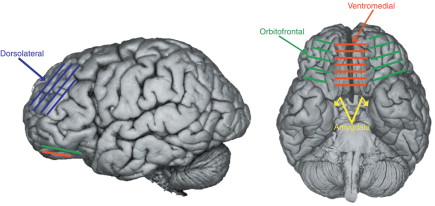
\includegraphics[width=0.7\linewidth]{pfc-brain-areas}
		%		\caption[PFC brain areas]{The PFC brain arreas. The illustration shows the physical location of the %dorsolateral cortex(blue color), the orbitofrontal cortex(green color) and the ventromedial cortex(red color) of the PFC. Also, the location of amygdala is illustrated with yellow color. The image is obtained from ...}
		%		\label{fig:pfc-brain-areas}
		%	\end{figure}
		There are also evidence that the PFC is involved with emotion processing and emotion regulation\cite{davidson2002anxiety,damasio1996somatic,balconi2012detection}. More specifically, the ventromedial prefrontal cortex is suggested to be involved in the representation of positive and negative emotional states, and the dorsolateral prefrontal cortex in the representation of the goal states towards these affective states are directed. Also, it is suggested that amygdala processes threat stimuli and processes negative affect of fear\cite{davidson2002anxiety}. Furthermore, the orbitofrontal cortex in the PFC has been linked to reward processing and reinforcement learning\cite{rolls2000orbitofrontal}, therefore playing a role in the assignment in emotional valence and intrinsic motivation.
		
		Davidson proposed the ``valence asymmetry hypothesis''\cite{davidson1992emotion} which states that positive affect which is linked to approach motivation is experienced when the left frontal cortical region has higher activation than the right. In contrast, negative affect which is linked to avoidance motivation is experienced when more activation is observed in the right frontal cortical region compared to the left. However, the valence model of emotions by Russell\cite{russell2003core} does not connect emotional valence with approach-avoidance motivation because the emotional state of anger. Consequently, we are interested in using fNIRS in order to measure the activations in left and right frontal hemispheres and interpret the results using the \textit{valence asymmetry hypothesis}. We will review more relative studies that used fNIRS to investigate the relationship between left and right hemispheres in the ``fNIRS and Emotional Valence'' subsection below. 
		
		\subsection{Fnirs and mental workload}
			In this subsection we review studies that used fNIRS in cognitive tasks. To begin with, fNIRS has been placed in different brain regions like, prefrontal cortex\cite{ayaz2012optical}, motor cortex\cite{hirth1996non} and auditory cortex\cite{plichta2011auditory}. However, because a positive correlation has been observed between the hemodynamic data from the prefrontal cortex and mental workload\cite{parasuraman2005neural} we review only studies that are measuring PFC hemodynamic activation. 
			Generally, fNIRS has been used in various tasks, including remotely operating vehicles\cite{durantin2014using,ayaz2012optical}, mental arithmetic\cite{pike2014measuring}, n-back tasks\cite{durantin2014using,ayaz2012optical}, and other complex cognition tasks like video games\cite{izzetoglu2004functional,bunce2011implementation,ayaz2012optical}. However, those studies measure whether there is difference in the hemodynamics between conditions when changing the difficulty of the tasks. According to our knowledge there is only one study using fNIRS for evaluation of desktop visualisation interfaces, and more specifically comparing bar graphs and pie charts\cite{peck2013using}. They tested 16 participants, however, they could not find statistically significant difference in Hbr activation between the two graphs.
			Furthermore, it has been suggested that Hbo activation tends to be more sensitive compared to Hbr and Hbt during  mental task\cite{naseer2014online}. Another study by Plichta et al.\cite{plichta2006event} studied the reliability over time of the hemodynamic data from fNIRS and concluded that Hbo data was more reliable and stable than Hbr data. Therefore, we will use primarily Hbo for inferring mental workload and emotional valence, although Hbr and Hbt data will still be examined and results reported.
			
					
			%Remotely operated vehicles \cite{durantin2014using,ayaz2012optical}
			%Working memory task (n-back task\cite{durantin2014using,ayaz2012optical}, mental aritmentic\cite{pike2014measuring})
			%Video game task Warship commander task\cite{izzetoglu2004functional,bunce2011implementation}
			%video game air traffic controller\cite{ayaz2012optical}
		\subsection{fNIRS and emotional valence}
			In this section we review studies that use fNIRS data to infer about affective states measuring the hemodynamic activity of the PFC. It was not found a usability study incorporating fNIRS for measuring emotional valence. Most of the research papers use a set of predefined pictures, videos, face expressions, and words to induce positive or negative emotions.
			
			Most of studies use a set of affective pictures\cite{lang1997international} to elicit emotion. Balconi et al.\cite{balconi2015hemodynamic} used multiple measures from fNIRS, EEG, skin conductance, and heart rate showed affective pictures to test the valence asymmetry hypothesis. They also used the SAM subjective questionnaire to relate the psychophysiological to the self reported one. The measured Hbo from the fNIRS in the frontal right hemisphere was significantly higher when negative pictures were presented to participants. Moreover, the EEG and skin conductance data yield equivalent results. Also, it was found out that negative stimuli were more arousing according to the data from skin conductance measure. Generally, the results from this study were in accordance to the valence asymmetry hypothesis.	Another study found that positive happy face expressions were identified faster and the reaction times were lower compared to negative or angry expressions\cite{root2006left}. Also, right handers reacted faster to positive face expressions with their right hand, and to negative expressions with their left hand. The opposite pattern was observed for the left handers which reacted faster to positive stimuli with their left hand and to negative with their right hand. A similar study\cite{kong2013space} used words and facial expression to induce affect, and yield identical results as the previous one. This supports the body-specificity hypothesis\cite{casasanto2009embodiment} which states that right handers associate positive emotions with their right hand and negative emotions with their left hand. The and opposite pattern should be observed for the left handers. Consequently, it left-handers and right-handers will activate different areas of the brain viewing the same affective stimuli. Taking in consideration the limited time we have for this master thesis, and the need for significant statistical difference, we should study either right-handed or left-handed individuals.
			
			Furthermore, a study showing a emotional video clips\cite{leon2006differential} to participants deducted that there was a gender difference in the delay period to initial PFC activation. Later, the same authors made a similar experiment \cite{leon2007lasting} using video clips to elicit affect found out that there was activation even after finishing the video clip and the off periods should be adjusted so that post-stimuli activation do not overlap with the next condition.

			However, the above mentioned studies are designed to induce emotions, but want to study the opposite effect: can we obtain emotional valence rating from neutral web interface using fNIRS, and then infer which of the variations was objectively more preferred?

	\section{Summary}
		To sum up, many researchers do not consider the positive or negative affective state during task execution, and how it influences operator performance and perceived workload, we have combined multidimensional subjective workload scale (NASA-TLX) with emotional valence scale (SAM). We expect to gain better understanding of the operator performance and motivation during the web form filling task. Also, we expect to find correlations between these subjective measures and the objective measure of the mean Hbo from the fNIRS device because they are both suggested to measure mental workload and emotional valence. 

		
\chapter{User study}
	\section{Hypothesis and expectations}
	Based on the literature review we state the following hypothesis:\\
	1) There is significant statistical difference between the three web forms\\
	2) Subjective data from NASA-TLX correlates to objective data from the fNIRS\\
	3) The difference in left and right hemisphere activations correlate to subjective SAM scale of emotional valence\\
	
	We are aiming to reduce to imposed load by the task by minimizing the visual search(index3) and aiding the episodic memory by placing a description in the beginning of the web form(index2) compared to the control condition(index1). Thus, we expect to find differences between the three conditions. Because the number of attended cues affects the operator performance, we decided to split the web form into 3 pages, in order to minimize visual search and clutter. 
	
	Hypothesis 2 was drawn from the fact that both NASA-TLX and the mean Hbo data from fNIRS have been successfully used to measure the concept of mental workload, therefore, we expect to find correlations between the two measures.
	
	In addition, because fNIRS can measure the left and right hemisphere activation, which is correlated to positive and negative affect based on the valence asymmetry hypothesis, thus we can infer about the affective and motivational state of the participant. And also, hypothesis 3 was stated because the subjective SAM scale is valid measure for obtaining emotional valence(the affective state), we expect to find correlations between the SAM and left/right hemisphere Hbo activation.
	
	
	\section{Method}
	We have use fNIRS because it is non invasive, motion artefact resistant, and with high temporal resolution and, thus suitable for using in user trials. We combine the objective measure of fNIRS with the subjective NASA-TLX and SAM measures, as they are validated and reliable methods. This way we gather comprehensive information about how participants perceive the interfaces and relate it to the psychophysiological data. Also, using fNIRS is novel method for conducting usability studies, and we also, aim to assess its practicality in this kind of HCI evaluation studies.

		\subsection{Participants}
		A total of 20 right handed participants (9 female) with mean age of 26 (SD = 4.04) took part in the study. All of the participant were healthy, however only one pointed that it suffers ``Von Willebraud disease'' which impairs blood's ability to clot, and his data from the psychophysiological measures was excluded. All participants had normal or corrected to normal vision, and report no history of brain damage. Also, 14 of them reported they have advanced computer literacy, 5 of them stated average computer literacy and 1 did not answer this question. All of the participants were current or graduated students. The ethics committee of the University of Nottingham approved this study. Informed consent was obtained from the participants and they were compensated with £10 Amazon voucher.
		\subsection{Apparatus}
			\subsubsection{Laptop computer}
			The experiment was executed on 15" laptop, HP probook 450 with screen resolution 1366x768. An external mouse was attached, which participants used during the process. The participant was presented with a screen with links to the three different videos and web forms. They were instructed by the researcher to manually start certain condition or video. 
			\subsubsection{fNIRS}
			\hl{(Picture of fNIRS and emitter-detector pairs)-can I use the one from the TAP paper?}\\
			Hemodynamic data was recorded using the fNIRS300 device along with the COBI studio recording software developed by Biopac Systems inc. The device consists of a headband with 4 infrared LED emitters and 10 infrared detectors. They operated on 730nm and 850nm wavelengths. The combination between them was used to calculate 16 channels which can measure the associated Hbo and Hbr concentration in the PFC. The fNIRS device was placed on the forehead of the participants targeting the dorsolateral(BA 9/46) and orbitofrontal(BA 10) cortices.
			
        \subsection{Materials}
			\subsubsection{NASA-TLX}
			The NASA-TLX\cite{nasatlx} is multidimensional subjective scale and it is used as a tool for assessing operator workload based weighted average of its six scales. The individual scales are presented in the following order: Mental demand, Physical demand, Temporal demand, Performance, Effort, and Frustration. We used the paper version of the questionnaire. The NASA-TLX measures were obtained from participants each time after completing one of the web form conditions. We did not follow the weighting procedure because it was time consuming, and instead we calculated the mean values of all individual subscales, which is suggested to be also, a valid measure\cite{hart2006nasa}, and we refer to this variable as ``total tlx''. Furthermore, each of the individual subscales was analysed independently.
			\subsubsection{Self assessment manikin scale (SAM)}
			Self assessment manikin\cite{bradley1994measuring} is a two dimensional scale for measuring the perceived emotional valence and arousal. We implemented the 5 point version of it. The participants were asked to fill the questionnaire after each video watched and each web form filled. First they state their emotional valence(negative or positive) by choosing between 1 and 5, where 5 is strongly perceived positive emotion, and 1 is considered strong negative emotion. Then, they fill the arousal level scale, where 1 indicates low perceived arousal or boredom, and 5 signifies high perceived arousal or high level of excitement. Each of the subscales is supported by image visualisations illustrating the affective state.
			\subsubsection{Web forms}
			A total of 3 HTML/CSS variations of a standard web form for insurance claiming were produced. They were created to resemble an actual online insurance claim form. All of the conditions were divided on 3 main divisions: Personal information, Accident information and Summary of accident. The personal information division consisted of 5 individual forms, namely: First name, Last name, Date of birth, Email, You are(choose type of stakeholder, which was option field). The accident information consisted of one text input field(Today's date), four drop down lists(Number of passengers, Number of cars involved in the accident, Was anyone injured in this incident, and Was the accident caused by your fault), and a checkbox form for selecting which areas of the vehicle were damaged. Lastly, the third division consisted of a text-area, where participants had to write a description of the accident. The first version or the control version, referred as index1, consisted of the 3 division areas laid out in the order that was described here, namely, at the top of the page is the personal information, followed by accident information and lastly summary of accident. In the second web form, which we refer to as index2, the summary of accident area was placed on the top of the page, followed by personal and accident information, accordingly. The third condition, referred as index 3 had the same order as index1, however each division area was situated on separate page, and consisted of total 3 pages. Users navigated between the three pages using a submit button with the label``Next''. Also, on the top of the form below the heading there was a progress feedback text indicating of how many steps the web form consisted. For more detailed information, the three web form conditions can be viewed in \hl{Appendix number}
			\subsubsection{Video capture}
			A video capture of the computer screen was recorded during the experiment using Fraps\cite{fraps}. The participants voice was recorded too. The timestamp of the beginning of the video recording was obtained, in order to be able to calculate duration of tasks, and their actual start and end time.
			\subsubsection{Video clips of auto accidents}
			
		\subsection{Design}
		The study used repeated measures within subjects design. The depended variable was the \hl{task completion time(or user preference)}, and the independent variable was the layout of the three web forms. The control condition was index1. Before the start of each web form, a video of road accident was played. The three variations of videos and the web forms were counterbalanced using latin square rotation, in order to avoid learning effects from the order of presentation of the video clips.
		\subsection{Procedure}
		\begin{figure}[h]
			\centering
			\includegraphics[width=0.95\linewidth]{"study-procedure"}
			\caption[study procedure]{The image illustrates, the study procedure followed in this experiment. First participants, watched video, then fill the SAM measure. After that, they filled the a web form, and then filled both the NASA-TLX and SAM scales. The process was repeated 3 times.}
			\label{fig:study-procedure}
		\end{figure}		
		Participants followed the procedure illustrated by Figure\ref{fig:study-procedure}. First, participants were asked to read and sign information sheet and consent forms. Second, the fNIRS device was cleaned then equipped and started. Third, participants were briefed about the procedure of the experiment, and it was explained how to fill the subjective scales. Also, because of ethical considerations that the participant should not enter personal data in the web form, a artificial personal credentials were provided, that she should fill in the web forms. Fourth, after the video capture and the fNIRS device were started, participants were asked to relax and try not to think about anything, in order to record a baseline of the hemodynamic activity in the PFC while participants are at rest. Next, they are asked to open one of the three videos, depending on the counterbalancing table. After the video was finished, participants fill SAM subjective scale. Fifth, there was approximately 2 minute waiting period between the video and the web form filling task, so that participant's memory is not fresh. Finally, after participant has completed the web form, the SAM and then the NASA-TLX scales are given to be completed, accordingly. This process was repeated three times, following the within subjects experimental design with counter balancing between the videos and the web forms. Because fNIRS device used one computer and the experiment was conducted on different computer, before each experiment, the clocks between the two computers were synchronized. Also, timestamps using the Cobi Studio software manual markers were created in the beginning and end of each condition and video. 
		\subsection{Data Analysis}
		The fNIRS data was analyzed with fnirsoft\cite{ayazfunctional}. Data from N=1 participant was excluded from the analysis because of ``von willebraud disease'' which is known to alter the signal. Also, data from another N=8 participants was excluded due to the fNIRS apparatus not able to detect signal from the channels for those participants. When calculating the correlation between fNIRS data and other measurements we excluded the data from these 9 problematic participants from the subjective or performance measures accordingly.
			\subsubsection{Signal acquisition}
			The fNIRS headband was placed on participants forehead, targeting the prefrontal cortex. The emitter-detector separation was 2.5cm and the sampling rate was 2Hz.
			\subsubsection{Preprocessing}
			Instrument noise was reduced by placing a hat over the fNIRS headband, in order to block external light.
			First, low-pass filter with cut off frequencies of 0.1 Hz, was used in order to remove physiological noise, like heartbeat and blood flow movement that is not associated with brain activity or Mayer waves.
			Then, the NIRS signal was processed with modified Beer-Lambert law\cite{cope1988system}, in order to calculate oxygenated, and deoxygenated hemoglobin values.
			Finally, to remove motion artefacts, the correlation based signal improvement(CBSI)\cite{cui2010functional} method was applied to the data.
			\subsubsection{Feature Extraction/selection}
				\paragraph{fNIRS mean Hbo, Hbr, and Hbt data}\leavevmode\\
				After data preprocessing the mean, and standard deviation for Hbo, Hbr and Hbt data was calculated from all channels, in order to infer about activation in the participants PFC. Hbo has been suggested to positively correlate to mental workload, in contrast to Hbr which is proposed to have negative correlation to mental workload.
				\paragraph{fNIRS mean differences}\leavevmode\\
				To calculate the left versus right hemisphere activation from the fNIRS we subtracted the mean data from channels 1-8, which are situated at the left side of the participants PFC, from the mean data of channels 9-16 which are on the right side of the PFC. That gave us the difference value between the left and right hemisphere. It indicates that the higher the mean difference value the more positive affect or affordance motivation the web form elicited. And the opposite pattern: the lower the mean difference the more negative affect or avoidance motivation the participant experience according to the valence asymmetry hypothesis.	
	\section{Results}
		\subsection{Mental Workload}
			\subsubsection{fNIRS data}
			A one-way repeated measures ANOVA was conducted to determine whether there was a statistically significant difference in mean Hbo values between the three web forms. The assumption of sphericity was met, as assessed by Mauchly's test of sphericity, $X^{2}(2) = 0.195, p = 0.907$. There was no significant statistical difference in the mean Hbo between the 3 web forms  $F(2,20)=3.400, p<.054,$ partial $\eta^{2}=.254$ with mean Hbo decreasing from 0.2377 (SD = 1.19) in index3 to -0.1166 (SD = 0.82) and -0.117 (SD = 1) for index2 and index1 respectfully. Which means that index3 indicates the highest workload, compared to the rest of the conditions.
			\begin{figure}[h]
				\centering
				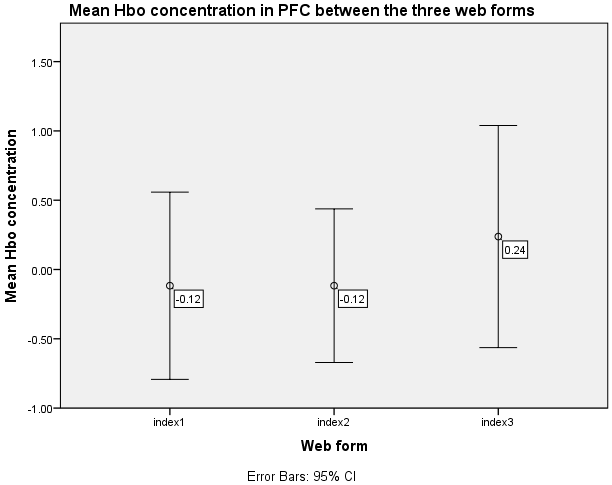
\includegraphics[width=0.7\linewidth]{mean-hbo-index123}
				\caption[mean Hbo activation between the three web forms]{Mean Hbo activation between the three web form conditions as measured by fNIRS. Higher Hbo values indicates higher mental workload experienced by the operator.}
				\label{fig:mean-hbo-index123}
			\end{figure}
			After conducting t-tests between index1 and index3 there was found a marginal statistical difference p=0.054. Which means that the measured Hbo between the two versions has a 94.6\% statistical probability that the difference are not caused by random sampling error. However, we fail to reject the first null hypothesis. This means that we could not find a statistically significant interaction, however we were very close to statistical significance, as p=0.054 and we can assume we have marginal statistical significance.
	
			Also, no statistical significance was found when comparing the means of Hbr between the three conditions $F(2,20)=2.044, p<.156,$ partial $\eta^{2}=.170$ where index2 had the highest Hbr mean 0.05 (SD = 0.85), index1 with -0.07 (SD = 0.96) and index3 with the lowest Hbr mean -0.36 (SD = 1.43). Which, accordingly negatively correlated to Hbo data, and again indicated that index3 evoke the highest workload than the other conditions. Furthermore, a repeated measures ANOVA test was conducted to elicit significant statistical differences between mean Hbt between the three web forms, however no statistical significance was found $F(2,20)=0.685, p<.516,$ partial $\eta^{2}=.064$ where index2 had the highest Hbt mean -0.08 (SD = 0.49), index3 with -0.13 (SD = 0.58) and index1 with the lowest mean Hbt -0.19 (SD = 0.49). The results indicate that Hbo was more responsive for this experiment and gave us higher significance between condition compared to Hbr and Hbt. 
			No correlation was found between the fNIRS mean data and any of the NASA-TLX scales, including the calculated total tlx. As a result, we fail to reject the second null hypothesis which states there is no difference between objective data from fNIRS and subjective data from NASA-TLX.
			\subsubsection{NASA-TLX}
				We report data for the NASA-TLX measure for all of the participants without excluding anyone because there was no problem with obtaining the data for this measure. All of the calculated data can be viewed in Table \ref{nasa-tlx}.
				There was no statistical significance between each of the NASA-TLX scales, including the total$F(2,38)=0.743, p<.482,$ partial $\eta^{2}=.038$ score as assessed by one way repeated measures ANOVA. Which means statistically we have 51.8\% chance of the results of the total NASA-TLX score to be caused by random sampling error. Also, perceived mean mental demand was lowest for index1 9.15 (SD = 4.94), index2 had slightly higher mean 9.40 (SD = 4.68) and index3 has the highest scores 10.8 (SD = 5.38). Also, mental demand had a strong positive correlation with total tlx for the 3 conditions $r(18)=0.652, p=0.002$, $r(18)=0.738, p<0.001$, and $r(18)=0.741, p<0.001$ for index1, index2 and index3 respectfully. Which supports the validity of NASA-TLX measurements. The total calculated value for the NASA-TLX was highest for index3 7.07 (SD = 3.22) decreasing to 6.92 (SD = 2.95) for index1 and 6.47 (SD = 3.11) for index2. This means that index3 requires slightly more attentional resources to complete the task compared to index1 and index2.
				There was a moderate positive correlation between mental demand scales and task completion times between the three conditions  $r(18)=0.487, p=0.030,  r(18)=0.484, p=0.030,  r(18)=0.638, p=0.002$. The results show that the more participants perceived higher workload the more their performance dropped as it took them more time to complete the task.
				
				\begin{table}[h]
					\centering
					\caption[NASA-TLX mean scores]{A table of all of the calculated mean NASA-TLX values for the 6 subscales, including the averaged total tlx}
					\label{nasa-tlx}
					\begin{tabular}{l|ccc}
						& Index1           & Index2           & Index3           \\[0.12cm]   \hline
						Mental demand   & 9.15 (SD = 4.94) & 9.40 (SD = 4.68) & 10.8 (SD = 5.38) \\
						Physical demand & 4.05 (SD = 4.08) & 2.90 (SD = 3.21) & 3.90 (SD = 3.65) \\
						Temporal demand & 7.40 (SD = 4.49)  & 7.65 (SD = 5.79) & 6.55 (SD = 4.91) \\
						Performance     & 6.65 (SD = 3.79) & 5.60 (SD = 3.62)  & 6.20 (SD = 3.86)  \\
						Effort          & 8.15 (SD = 4.58) & 7.35 (SD = 4.68) & 8.20 (SD = 5.30)   \\
						Frustration     & 6.10 (SD = 5.11)  & 6.00 (SD = 3.66)  & 6.75 (SD = 5.22) \\\hline
						Total 			& 6.92 (SD = 2.95) & 6.47 (SD = 3.11) & 7.07 (SD = 3.22)
					\end{tabular}
				\end{table}
	
			\subsubsection{SAM - arousal scale}
			As it can be seen from Figure~\ref{fig:sam-arrousal-index123} the perceived arousal was lowest for index1 2.8 (SD = 0.95) increasing to 2.95 (SD = 1.05) for index2 and to 3.15 (SD = 1.18) for index3 respectfully. No statistical significance was found when comparing the means between the three conditions $F(2,38)=2.462, p<0.099$ partial $\eta^{2}=.115$ using one way repeated measures ANOVA. However, after running post hoc test without adjustments(LSD) a statistically significant difference was found between index1 and index3 $p=0.049$. Which means that perceived arousal was significantly higher for index3 compared to index1.
			Also, the time to complete index1 and index2 positively correlated to perceived arousal for index 1 and index2:$r(18)=0.551, p=0.012$ and $r(18)=0.473, p=0.035$. However time to complete index3 does not correlate to perceived arousal of index3 $r(18)=0.269, p=0.252$. Which indicates that we have a partial positive correlation between the perceived arousal, which can be considered as workload, for the web forms and the time to complete them.
			
			\begin{figure}[h]
				\centering
				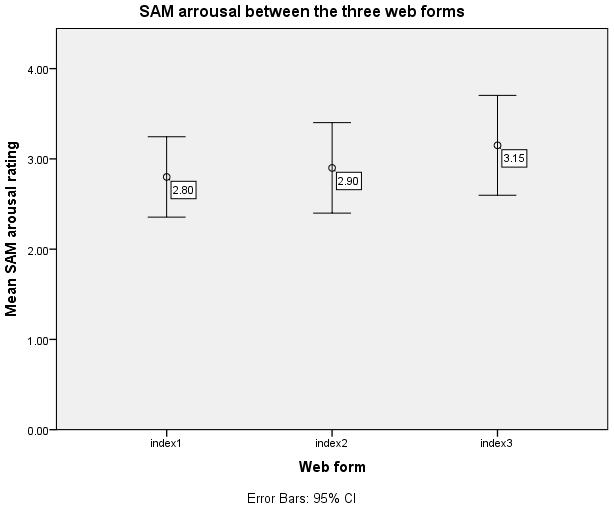
\includegraphics[width=0.7\linewidth]{sam-arrousal-index123}
				\caption[SAM arrousal between the three web forms]{The mean SAM arrousal rating obtained from the three web form conditions.}
				\label{fig:sam-arrousal-index123}
			\end{figure}
			
		\subsection{Emotional Valence}
			\subsubsection{fNIRS differences}
			\paragraph{Data from the period of web form filling}\leavevmode\\
				\begin{figure}[h]
					\centering
					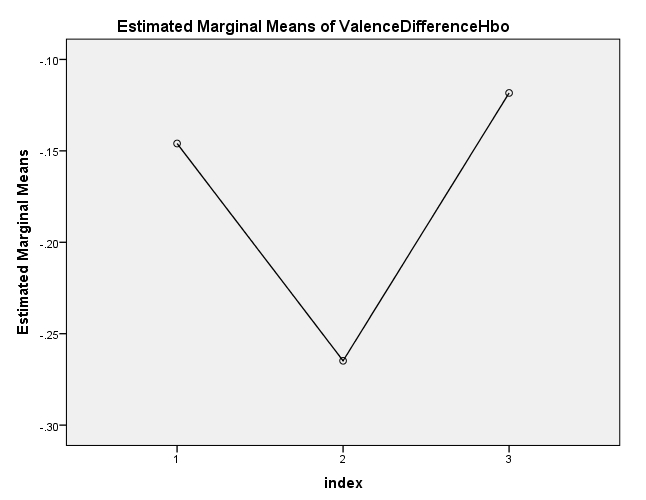
\includegraphics[width=0.7\linewidth]{hbo-valence-differences-index123}
					\caption[Hbo valence differences between the three web forms]{The mean Hbo valence differences obtained from the fNIRS for the three web form conditions. Higher values indicate more positive affect, and lower value more negative affect.}
					\label{fig:hbo-valence-differences-index123}
				\end{figure}									
				To begin with, Figure \ref{fig:hbo-valence-differences-index123} shows the valence differences in Hbo concentration between the left and right hemispheres. fNIRS Hbo valence differences was highest for index3 -0.12 (SD = 1.25) decreasing to -0.15 (SD = 1.31) for index1 and the lowest value was for index2 -0.26 (SD = 1.13). Indicating that participants experienced the most positive when completing the index3 condition, slightly less positive for index1 and the least positive when completing index2. However significant statistical difference was not found $F(2,20)=0.392, p<0.681,$ partial $\eta^{2}=.038$ as assessed by one-way repeated measures ANOVA.

				The Hbr valence differences were highest for index2 0.34 (SD = 1.18) decreasing to 0.18 (SD = 1.39) for index3 and to 0.10 (SD = 1.68) for index1. Signifying that index2 elicited the most negative affect compared to the rest of the conditions. However, the difference was not statistically significant.
				The Hbt mean valence difference values for index1 were lower -0.45 (SD = 0.79) compared to index2 0.06 (SD = 0.56) and index3 0.05 (SD = 0.87) respectfully. There was no statistical significance as assessed by one way repeated measures ANOVA between the three conditions for Hbr valence differences: $F(2,20)=0.418, p<0.664,$ partial $\eta^{2}=.040$ and Hbt valence differences: $F(2,20)=0.302, p<0.743,$ partial $\eta^{2}=.029$. Also, there was strong positive correlation between temporal NASA-TLX scale of index1 and the Hbo valence differences of index1 $r(9)=0.766, p=0.006$, however, there was no correlation found between index2: $r(9)=0.581, p=0.061$ and index3: $r(9)=0.218, p=0.519$ which suggests that as participants perceived more temporal demand the obtained mean Hbo data increased.\\
				
			\paragraph{Data from the period of video clips}\leavevmode\\
				The mean Hbo valence difference for video3 was the highest with 0.17 (SD= 0.25) compared to video1 with -0.01 (SD = 1.32) and video2 with -0.8 (SD = 1.20), suggesting that participants experienced more positive emotion when watching video3 compared to video1 and video2. In contrast, mean Hbr valence difference values for video3 were the lowest with -0.25 (SD = 0.47) compared to video1 0.30 (SD = 1.20) and video2 0.32 (SD = 0.89). For the mean Hbt valence difference values video1 was the highest with 0.18 (SD = 0.71) decreasing to 0.07 (SD = 0.64) for video3 and to -0.06 (SD = 0.35) for video2.\\
				A one-way repeated measures ANOVA was conducted to determine whether there was a statistically significant difference in Hbo, Hbr and Hbt valence differences between the three videos. There was no significant statistical difference in the mean Hbo valence difference between the 3 videos $F(2,20)=0.051, p<0.951,$ partial $\eta^{2}=.005$, the mean Hbr valence difference: $F(2,20)=0.062, p<0.940,$ partial $\eta^{2}=.006$ and the mean Hbt valence difference: $F(2,20)=0.522, p<0.601,$ partial $\eta^{2}=.050$. Consequently, we cannot find significant difference in the emotional valence from the objective data between the three videos.
				There was no correlation found between Hbo valence differences and SAM emotional valence subjective scale for the three videos $r(9)=-0.490, p=0.126$; $r(9)=0.095, p=0.781$; $r(9)=0.496, p=0.121$. As a result, we fail to reject the third null hypothesis, which states that there is no correlation between the fNIRS valence difference data and the SAM subjective scale of emotional valence.

			\subsubsection{SAM emotional valence}
			\paragraph{Data from the period of web form filling}\leavevmode\\
				The perceived mean emotional valence for index1 was the lowest with 
				3.1 (SD = 0.97) increasing to 3.4 (SD = 0.99) for index2 and to 3.7 (SD = 0.98) for index3, as it can be seen from Figure \ref{fig:sam-valence-index123}.
				\begin{figure}[h]
					\centering
					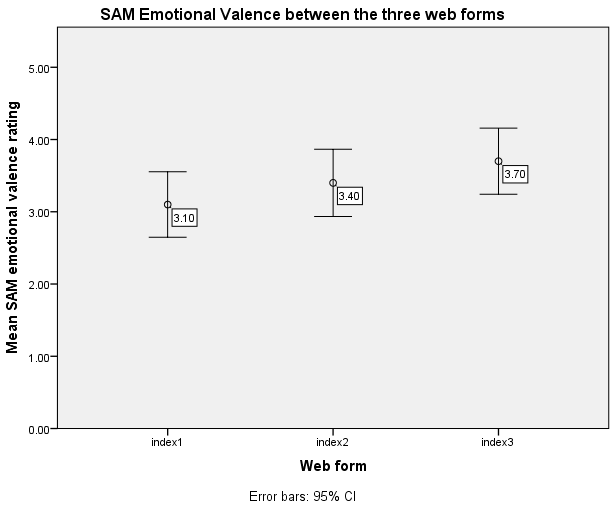
\includegraphics[width=0.7\linewidth]{sam-valence-index123}
					\caption[emotional valence between the 3 conditions]{Perceived emotional valence between the 3 web form conditions}
					\label{fig:sam-valence-index123}
				\end{figure}
				A one-way repeated measures ANOVA was conducted to determine whether there was a statistically significant difference in SAM emotional valence scale values between the three web forms. The assumption of sphericity was met, as assessed by Mauchly's test of sphericity, $X^{2}(2) = 0.446, p = 0.800$. There was no significant statistical difference in the SAM emotional valence scale between the 3 web forms  $F(2,38)=2.803, p<.073,$ partial $\eta^{2}=0.129$ with mean SAM emotional valence increasing from 3.1$\pm$0.97 in index1 to 3.4$\pm$0.99 and 3.7$\pm$0.98 for index2 and index3 respectfully. This means we cannot distinguish which web form participants perceived as more positive or negative, however we had marginal statistical significance which gives us high probability that the results were not being biased by random sampling error.	

			\paragraph{Data from the period of video clips}\leavevmode\\
				The perceived mean emotional valence for video3 was the highest with 3.1 (SD = 1.07) decreasing to 2.9 (SD = 1.33) for video1, and 2.7 (SD = 0.98) for video3. There was no statistical significance as assessed by one way repeated measures ANOVA between the three videos for SAM emotional valence: $F(2,38)=0.792, p<0.460,$ partial $\eta^{2}=.040$. The data suggest that we cannot compare the perceived emotional valence between the 3 video due to high chance of the results being caused by random sampling error.
		\subsection{User performance and preferences}
			\subsubsection{Task completion time}		
			\begin{figure}[h]
				\centering
				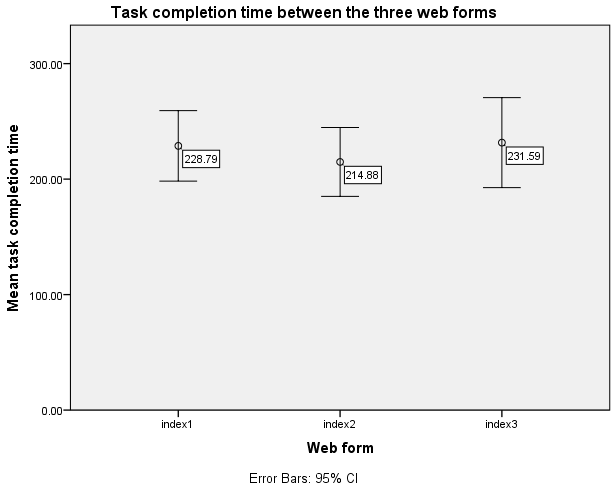
\includegraphics[width=0.85\linewidth]{mean-task-completion-time}
				\caption[Task completion time between the three web forms]{Mean task completion time between the three web forms}
				\label{fig:mean-task-completion-time}
			\end{figure}
			It can be seen from Figure \ref{fig:mean-task-completion-time} that the mean time to complete index2 was the lowest 214.88 (SD = 63.81) increasing to 228.79 (SD = 65.19) for index1 and to 231.60 (SD = 83.33) for index3. However, there was no significant statistical difference in time to complete between the 3 web forms $F(2,38)=0.556, p<.578,$ partial $\eta^{2}=.028$, as assessed by one-way repeated measures ANOVA. The results indicate that the performance was lowest when participants completed index3, slightly higher for index1 and the highest for index2.
			Also, the time to complete index2 and index3 had a strong positive correlation with perceived effort(NASA-TLX) for index2 and index3: $r(18)=0.702, p=0.016$ and $r(18)=0.634, p=0.036$. However, time to complete index1 does not correlate to perceived effort of index1 $r(18)=0.216, p=0.524$. This suggests that when participants perceived more effort it took them more time to complete the web form.
			\subsubsection{User preferences from the short-interview question}
			After the end of the experiment participants were asked which of the three web forms they prefer the most. The bulk of them preferred index3 and index1 with 10 and 9 votes respectively compared to index2 which was only preferred by 3 participants. The given answer were transcribed as can be seen in \hl{Appendix number}. 

\chapter{Discussion}
	\section{Comparison between the three web forms}
		\subsection{Index3}
		The purpose of this study was to improve usability of web form filling of insurance claims and find which of three web forms layouts was the most usable. After analysing the results we found out that index3 elicits the highest mental workload according to the fNIRS Hbo data which is correlated to workload, SAM arousal scale(significant difference with index1), total tlx, mental demand scale from NASA-TLX, and takes the most time to complete the task compared to the rest of the conditions. However, index3 was evoking highest positive valence(SAM), fNIRS differences were indicating more left hemisphere activation, and users preferred it the most when asked after the finish of the experiment. The results were unexpected according to the Norman\cite{norman2002emotion} positive affect should enhance operator creativity, thus increasing the performance, however we found the opposite results. 
		
		Also, it can be noted that perceived temporal demand for index3 was lower than index1 and index2(no statistical significance). This can be attributed to the fact that index3 had lower number of forms(visual cues) on each page. It can be inferred that the more web forms are present on an interface, the more the user feels temporal demand because it appraises the situation as one that needs more work to be performed. This claim can be supported with the feedback from the participants: \textit{``so the second one(index3) I felt having to click the links broke it down a little bit, like you didn't have to think about everything in one go...''} or other user expressed \textit{``you give all the details and then you take your time to write about the incident so you don't feel very rushed or something''}. 

		\subsection{Index2}
		Generally, index2 elicited the least workload inferred from the mean Hbo concentration, total tlx, perceived effort, physical demand, and frustration measures. Also, users performance was superior in index2, as the task completion time was the lowest, although not statistically significant. This can be attributed to the fact that index2 supported participants working memory better, specifically for this study design, because index2 presents the description field first, thus lowering the time to hold the visual information in the episodic memory. Consequently, users memory was relatively fresher when filling the description field in index2, which demanded the most attentional capacity, compared to the rest of the conditions. 
		
		Furthermore, index2 elicited approximately neutral emotional valence rating(3.40) which was higher than index1(3.10) and lower than index3(3.70). In contrast, the objective data from fNIRS differences reveal more right hemisphere activation which can be interpreted as more negatively valenced affect or avoidance motivation. The last finding can be supported with the fact that only 3 out of 20 participants expressed preference for index2. A possible explanation is that index2 did not support the consistency heuristic\cite{nielsen1990heuristic,shneiderman1992designing} because the description field is normally situated at the end of insurance claim forms. This statement can be supported by the following participant comments: \textit{``The only one I didn't like is the first one(index2) particularly. It was just describing the event before filling out the details it is a bit awkward.''}, and another participant stated:\textit{``Index1 and Index3 were Ok, but I didn't like index2 because I was not used to it.''}.
				
		\subsection{Index1}
		When analysing the results it can be noted that index1 was the least mentally demanding web form, according to the mental demand scale of NASA-TLX, and objective measure of mean Hbo activation, and the SAM arousal scale(statistical significance $p=0.049$ compared to index3). However, the calculated total tlx indicated higher perceived workload than index2, and lower than index3. Index1 can be said to support the consistency heuristic\cite{nielsen1990heuristic} because it was the control condition and represented a typical insurance claim form. The comparatively low workload measured for index1 can be attributed to the fact that the task was familiar, and therefore participants had to spending less working memory resources on planning because the task sequence was already mapped in the brain. One participant supported this argument by saying: \textit{``I consider it more logical, like logical approach..to say who you are, what happened to your car and then what happened exactly, describe it from your own perspective.''}. Also, 4 users reported that the sequence of small question first, leading to the description at the end, helped them to recall the situation better: \textit{``I preferred the first(index1) and third(index3) examples, as they asked more general questions at the beginning. This made me think about what aspects to include in the event summary at the end, such as number of cars involved''}. Which means that the sequence of web forms or their order of presentation is important aspect to consider.
		
		Furthermore, index1 induced the least perceived emotional valence from the SAM questionnaire, compared to the rest of the conditions, with marginal significance of $p=0.073$ when compared to index3. However, the objective data from the fNIRS differences demonstrated higher left hemisphere activation than index2, and slightly less than index3. Similarly, it took more time to complete the web form compared to index2, and slightly less time than index3.
				
		\subsection{Divided vs single page approach}
		A division can be made between the web forms which contain all forms on one page(index1, index2), and web forms which are consolidated or divided on several pages(index3). We define these as the \textit{single page approach}, and the \textit{divided page approach}, respectively.
		
		A possible explanation of the higher measured positive emotional valence across all measures for the divided page approach is that users had to process less informational cues at a time, compared to the single page approach, which they appraise as a positive experience. As one of the participants mentioned \textit{``because you don't have to think about the other forms''}. So having less web forms displayed on one screen improves visual search, decreases clutter, which imposes less temporal demand on the task. Consequently, users appraise the task as more positively valenced because it spends less attentional resources for meta-cognition.
		
		One advantage of the single page approach is that participants can go back and check what information they have already entered: \textit{``I remember in the second one(index1) I'm not sure whether the option provided left or right, so I rechecked''}. This way working memory resources are saved because participants has the ability to quickly recheck what they have already entered, relying on recognition, rather than recall\cite{nielsen1990heuristic} from working memory the same information again. Another advantage of the single page approach is that participants can choose which form to start first: \textit{``the good thing about the number two(index1) is everything is on the same page I can choose whatever I like''}. Generally, some of the participants preferred to fill in the description field first, and then the rest of the forms, so researchers and practitioners have to give users the power to choose from where to start. However, in our case the participants watched a recorded accident that they had to recall after approximately 2 minutes. In reality, the delay between the accident and the claim form filling will be much higher, thus the arrangement of the web forms depends on the time between the accident and the claim form filling.
		
		If we have to choose which of the web forms we should implement, in our opinion, index1 is most suitable because it elicited less mental workload in 3 out of 4 measures for workload, and the 10 out of 20 users expressed that their prefer it.	Also, index1 met the consistency heuristic, it gave more control and freedom to the user by letting her choose from which form to start first. 	
		Also, index3 should also be considered because it produced most positive valence according to our subjective(SAM) and objective(mean Hbo differences) measures. In addition, 11 out of 20 users favoured this web form.
				
	\section{fNIRS and valence asymmetry hypothesis}
	Unfortunately, we could not prove the valence asymmetry hypothesis\cite{davidson1992emotion} because we had no power and statistical difference for both, the videos and the web forms. We also, could not find a correlation between SAM emotional valence scale and the mean Hbo differences between the left and right hemispheres. One of the reasons we could not obtain statistical significance is that we followed the opposite approach to what other studies did. They used already researched and proven frameworks which contain previously classified affective stimuli while we present them with an unclassified interface which was not previously evaluated as neither positive and negative, and tried to infer about the emotional valence based on the valence asymmetry hypothesis. Unfortunately, we obtained far from significant difference between the three conditions $p=0.681$. This suggests that the approach we took requires testing with more participants. Which is not suitable for real life HCI evaluation studies because the limited time availability for such projects.
	
	\section{fNIRS practicality for HCI evaluations}
		One of the aims of the study was to assess the feasibility of fNIRS for HCI evaluation studies. After analysing the fNIRS data from 20 participants we had to exclude 9 because of bad data. However, we were close to reaching statistical significance between the three conditions as the p value was $p=0.054$ with only 11 subjects examined. This gives promising results that fNIRS can be used as reliable objective measure for workload in usability studies. We propose that a study needs approximately 20 participants, in order to reach statistical significance, however that is four times more than the suggested 5 users tests by Virzi\cite{virzi1992refining}. It should be noted that this recommendation highly depends on study design, and some studies may require only 10 subjects, while others more than 30.
		Other advantage of fNIRS is that it provides continuous measure of the Hbo concentration in the PFC, thus it can be highly suitable for detecting distinct periods of overload. For example, it can be particularly useful in game studies where participants should stay in the flow\cite{nakamura2002concept} state. Also, functionally the flow experience has been suggested to be situated in the prefrontal cortex and medial temporal lobe\cite{dietrich2004neurocognitive}, consequenly fNIRS can be used to measure it. As a result, researchers should be able to detect moments where the challenge of the game is either too difficult or too easy.
		When considering the measurement of emotional valence by comparing the hemodynamic activation between the left and right hemispheres was can conclude that we were unsuccessful as we were far from statistical significance($p=0.681$). More focused research should be conducted in order to test this approach. 
	\section{Implications for Design}
		- Include visual representations of information where possible, rather than display it as text only.
		- Sequence of web forms is important aspect to consider, so testing the order of presentation of forms may yield important information about 
		
	\section{Disadvantages of the study}
		The study tries to simulate real conditions, and therefore lacks ecological validity because users wait approximately 2 minutes after they have watched the video to start filling the web form. This way they still hold some of the information in their working memory and the study is trying to simulate long term memory recall.
		
		One of the disadvantages of near infrared scanning technology is that, in order to collect reliable measurements the emitter-detector pairs have to be in contact with the skin constantly, which causes pain and discomfort, after approximately 40 minutes of wearing the device.
	\section{Future work}
		
	\section{Conclusion}
		In summary, the mental workload is lower for this...
	\addcontentsline{toc}{chapter}{References}
	\bibliographystyle{plain}
	\bibliography{exmplref}
	\addcontentsline{toc}{chapter}{Appendix}
\chapter*{Appendix}
\end{document}